\documentclass[11pt, a4paper]{article}
\usepackage{a4wide}
\usepackage{amsmath, amsfonts, dsfont, booktabs, graphicx, natbib, a4, times, microtype, hyperref}
\newcommand{\E}{\ensuremath{{\mathbb E}}} % expected value
\def\func#1{\mathop{\rm #1}}
\begin{document}
\title{Solution to Exercise 7}
\author{Simon A.\ Broda}
\date{}
\maketitle

\begin{enumerate}


\item
\begin{enumerate}
\item If the relative price of oil expressed in units of gold, $\mbox{oil}_t/\mbox{gold}_t$, is stationary, then this implies that $\log(\mbox{oil}_t/\mbox{gold}_t)=\log (\mbox{oil}_t) - \log(\mbox{gold}_t)$ is also stationary, so $\log(\mbox{oil}_t)$ and $\log(\mbox{gold}_t)$ must be cointegrated with cointegrating vector (1, -1) if the individual series are integrated.
\item We begin by transforming the data to logs and making a plot:
\begin{verbatim}
genr lgold = log(gold)
genr loil = log(oil)
\end{verbatim}

Plotting the data requires opening the two series as a group. The resulting plot is given below.
\begin{center}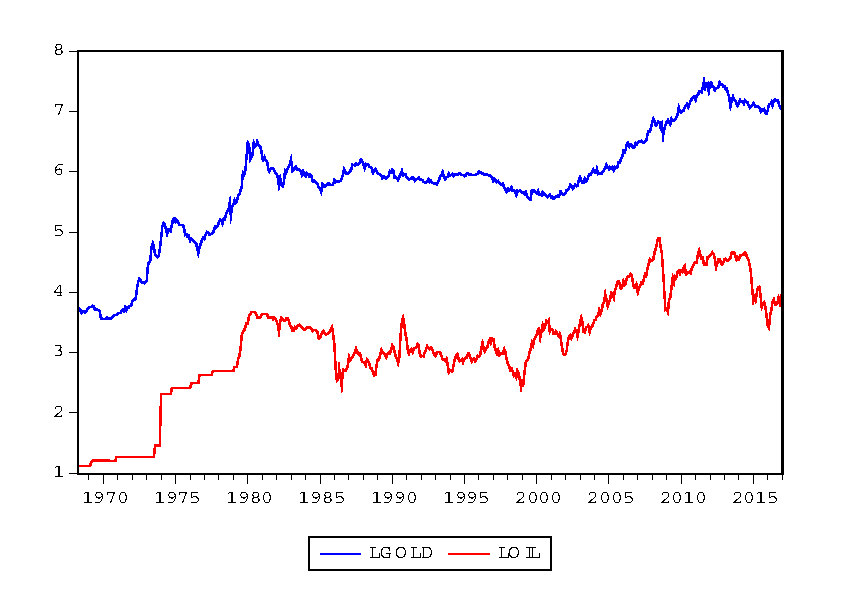
\includegraphics[width=0.7\textwidth]{oilgold2017}\end{center}

Then we follow the Engle-Granger procedure.

\noindent\textbf{Step 1}: Conduct individual unit root tests to make sure both series are integrated. We include a time trend for both because the data look trending, and choose the lag length automatically by the AIC.
\begin{center}
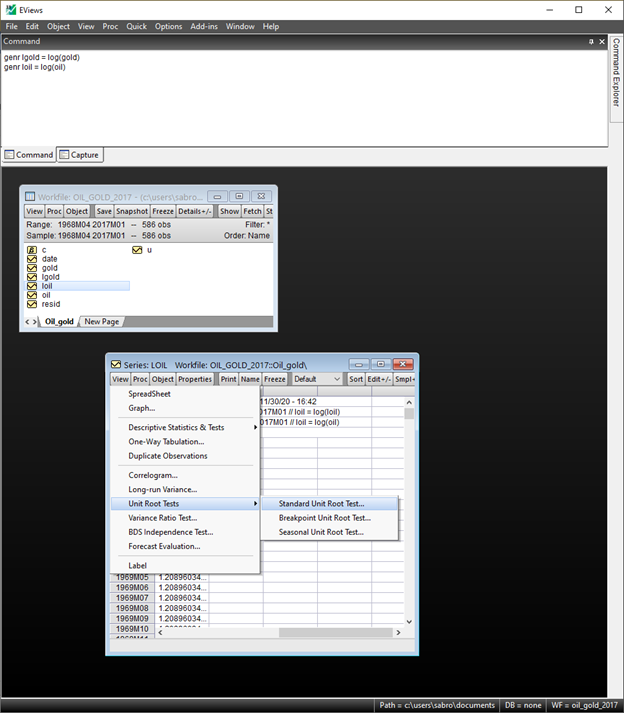
\includegraphics[width=.8\textwidth]{adfeviews}
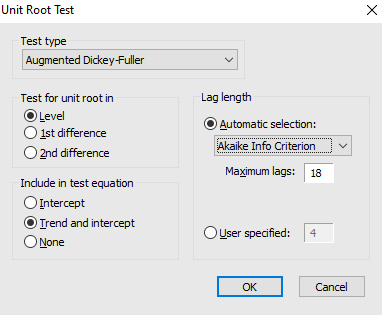
\includegraphics[width=0.4\textwidth]{adfeviews2}
\end{center}

The results is shown below.
\begin{center}
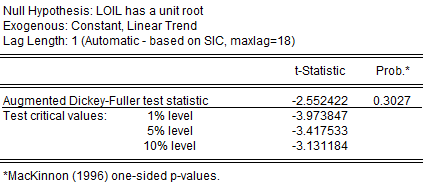
\includegraphics[width=0.6\textwidth]{ADF_loil}
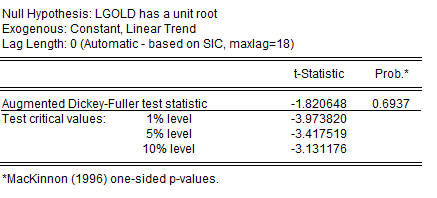
\includegraphics[width=0.6\textwidth]{ADF_lgold}
\end{center}
EViews chose to include one lagged difference. Neither test rejects, so the series are I(1).

\noindent\textbf{Step 2}: Estimate the long-run relationship (cointegrating relationship)
\[
\mbox{loil}_t=\beta_1+\beta_2\mbox{lgold}_t+U_t.
\]
\begin{center}
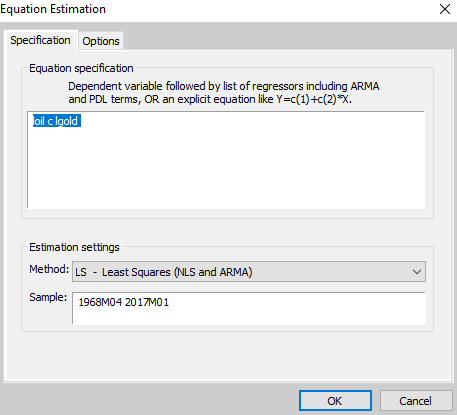
\includegraphics[width=0.6\textwidth]{longruneviews}
\end{center}
The result is
\begin{center}
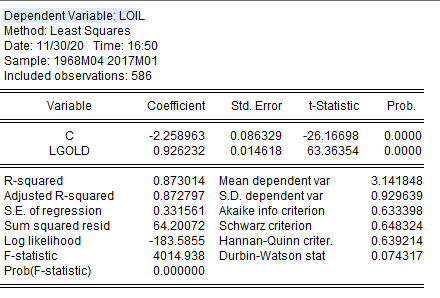
\includegraphics[width=0.6\textwidth]{longrun}
\end{center}
The estimated long-run relationship is
\[
\mbox{loil}_t=-2.26+0.926\mbox{lgold}_t+U_t.
\]
The estimated cointegrating vector (provided we find cointegration) is $(1, -0.926)$, i.e.,  \[\mbox{loil}_t-0.926\mbox{lgold}_t=-2.26+U_t\] is stationary. We save the residuals for later use and plot them:
\begin{center}
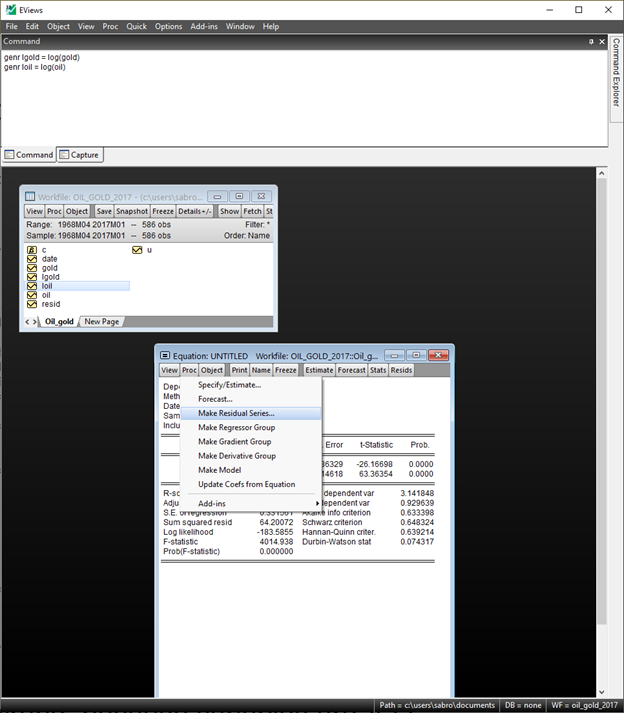
\includegraphics[width=0.8\textwidth]{residualseviews}
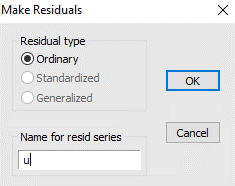
\includegraphics[width=0.4\textwidth]{residualseviews2}
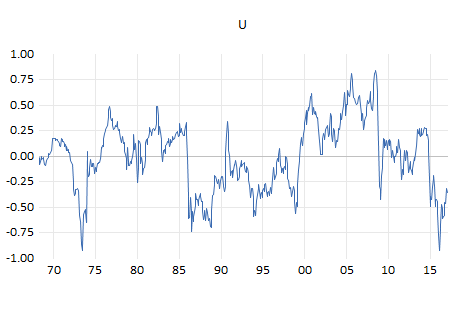
\includegraphics[width=0.6\textwidth]{residuals}
\end{center}

\noindent\textbf{Step 3}: Conduct an ADF test (with just an intercept, no trend!) for the residuals to test $H_0:$ No Cointegration. Result:

\begin{center}
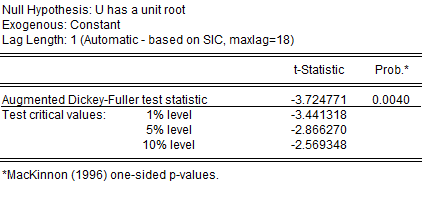
\includegraphics[width=0.6\textwidth]{englegrangertest}
\end{center}

Be careful to use the Engle-Granger critical value of -3.41 at the 5\% level. The test rejects the null. Conclusion: there is indeed cointegration.

Alternative to this manual approach: select \texttt{loil} and \texttt{lgold} (click on one, press control, click on the other), and open them as a group. Then do
\begin{center}
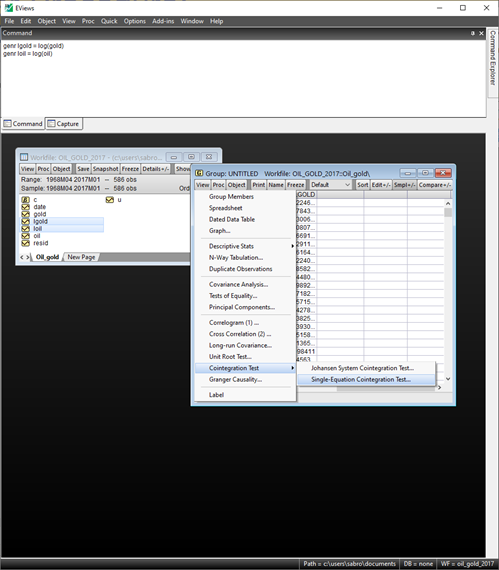
\includegraphics[width=0.8\textwidth]{englegrangereviews}
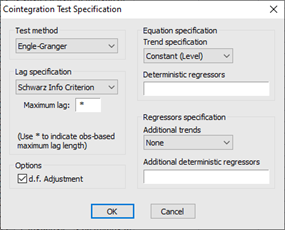
\includegraphics[width=0.4\textwidth]{englegrangereviews2}
\end{center}
Result:
\begin{center}
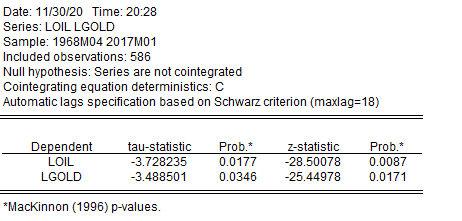
\includegraphics[width=0.6\textwidth]{englegrangereviews3}
\end{center}
Same result (first row), and we even get a $p$-value! Note that EViews does the test ``in both directions'', once with $Y_t$ as dependent variable and once with $X_t$. As mentioned in the slides, this doesn’t matter asymptotically, but in finite samples it might matter which of the variables we consider endogenous and which one exogenous. In this particular case though, they both give the same answer. Still, it would be better not to have to make a choice here. That’s what the Johansen procedure accomplishes.


\noindent\textbf{Step 4}: Estimate the VECM
\begin{eqnarray*}
\Delta Y_{t} &=&c_1+\alpha _{1}(Y_{t-1}-\beta _{1}-\beta _{2}X_{t-1})+e_{1t}, \\
\Delta X_{t} &=&c_2+\alpha _{2}(Y_{t-1}-\beta _{1}-\beta _{2}X_{t-1})+e_{2t}.
\end{eqnarray*}
replacing $Y_{t-1}-\beta _{1}-\beta _{2}X_{t-1}$
by the OLS residual $\hat{u}_{t-1}=Y_{t-1}-\hat{\beta}_{1}-\hat{\beta}_{2}X_{t-1} $ we saved earlier. Then, we can estimate $\alpha _{1}$ and $\alpha _{2}$ by OLS. We start with the equation for \texttt{LOIL}:
\begin{center}
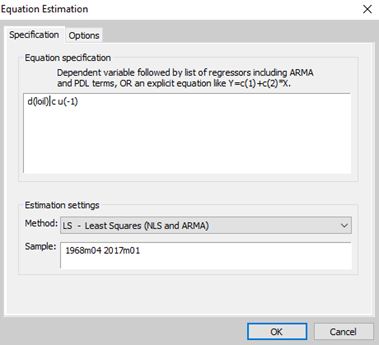
\includegraphics[width=0.6\textwidth]{vecmeviews}
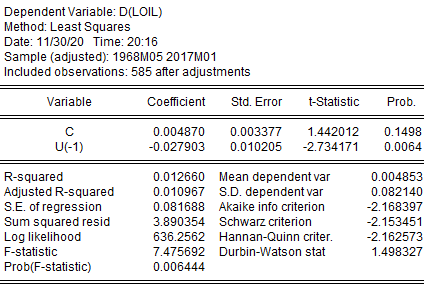
\includegraphics[width=0.6\textwidth]{vecm0}
\end{center}
We notice that there is autocorrelation (look at the DW stat). We can cure this by adding a lagged difference (like the ADF test did automatically when it selected the lag length).
\begin{center}
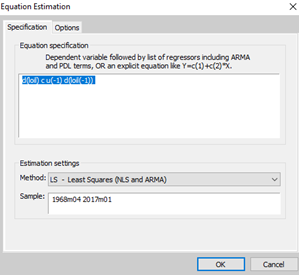
\includegraphics[width=0.6\textwidth]{vecmeviews1}
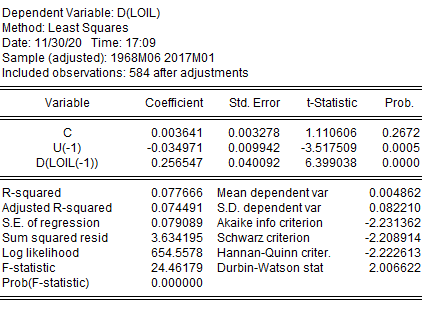
\includegraphics[width=0.6\textwidth]{vecm1}
\end{center}
Now it's fine. Let's repeat for the other variable:
\begin{center}
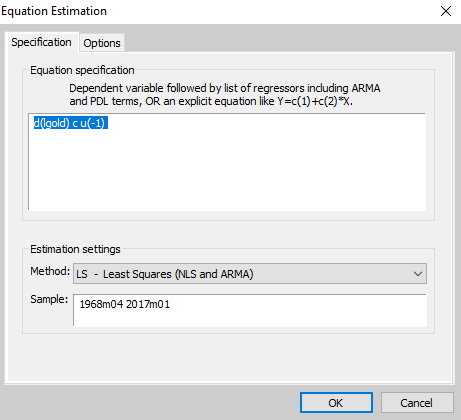
\includegraphics[width=0.6\textwidth]{vecmeviews2}
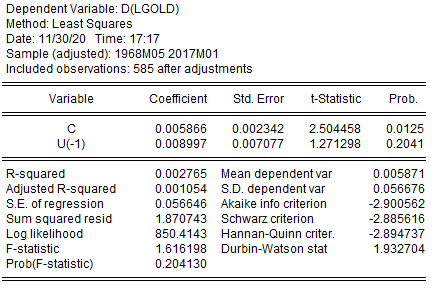
\includegraphics[width=0.6\textwidth]{vecm2}
\end{center}
This one seems fine without any lagged differences. We notice that $u_{t-1}$ is insignificant, so we can stick with a single-equation ECM. The final model is
\[
\Delta \textrm{loil}_t=0.0036-0.035(\textrm{loil}_{t-1}-0.926\textrm{lgold}_{t-1}+2.26)+0.25\Delta\textrm{loil}_{t-1}+e_{1t}
\]
Interpretation: there is an equilibrium relationship between \texttt{loil} and \texttt{lgold}, with cointegrating vector $(1, -0.926)$. In case of a disequilibrium, \texttt{loil} adjusts towards the equilibrium. The
adjustment amounts to 3.5\% of the disequilibrium per period.
\item We now repeat the analysis, but using Johansen's procedure, rather than Engle and Granger's. \\
\noindent\textbf{Step 0} The first step is to pick a lag length. In slides, we didn't do this: we just picked a lag length of 1 because that's what we used in the Engle-Granger procedure. If we hadn't done Engle-Granger and started with Johansen right away, we'd need a way to do this.
The easiest way is the following: open the variables as a group like before, then click on \texttt{Proc$\rightarrow$Make Vector Autoregression}.
\begin{center}
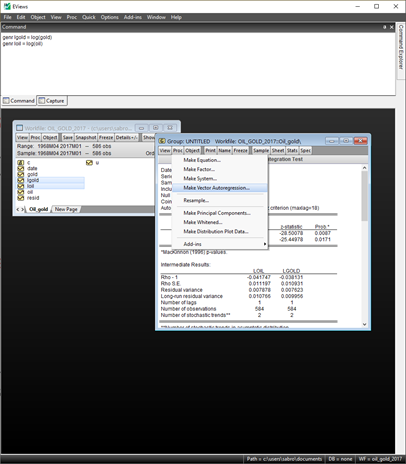
\includegraphics[width=0.8\textwidth]{johanseneviews1}
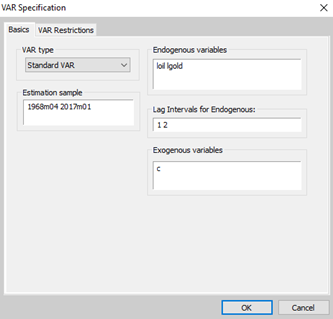
\includegraphics[width=0.4\textwidth]{johanseneviews2}
\end{center}
Keep the defaults, hit enter, and ignore the output. We're just doing this to get to the multivariate information criteria, by clicking \texttt{View$\rightarrow$Lag Structure$\rightarrow$Lag length criteria}:
\begin{center}
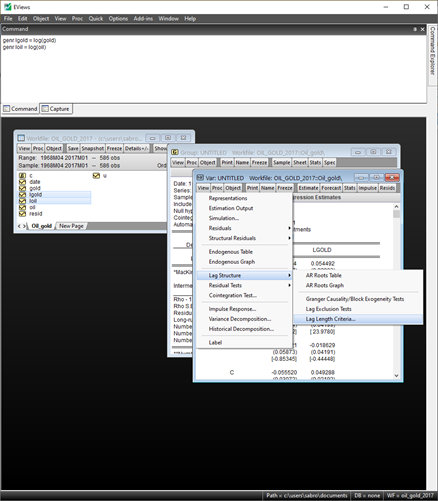
\includegraphics[width=0.8\textwidth]{johanseneviews3}
\end{center}
This yields
\begin{center}
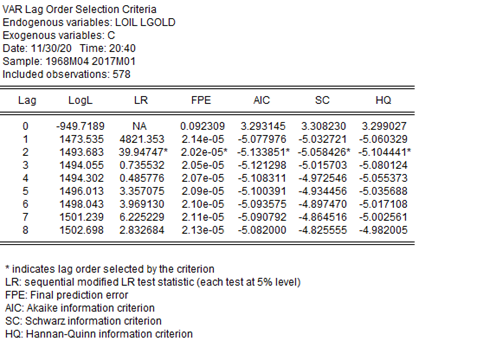
\includegraphics[width=0.6\textwidth]{johanseneviews4}
\end{center}
Most criteria agree on 2 lags. For technical reasons (this is a VAR, not a VECM), this means that we need 1 lag in the Johansen test and in the VECM.\\
\noindent\textbf{Step 1} Conduct the Johansen test. Open the variables as a group as before, then do
\begin{center}
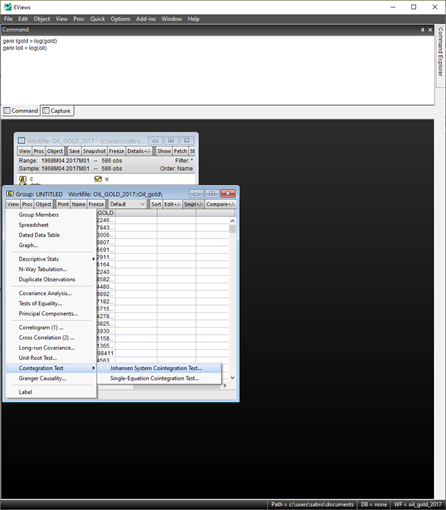
\includegraphics[width=0.7\textwidth]{johanseneviews5}
\end{center}
Choose Option 3 to allow for a trend, and specify the lag interval as \texttt{1 1} (this means all lagged differences from lag 1 to lag 1), because that is what the information criteria suggested.
\begin{center}
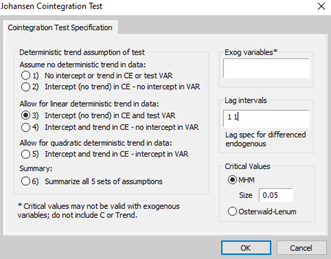
\includegraphics[width=0.4\textwidth]{johanseneviews6}
\end{center}
Result:
\begin{center}
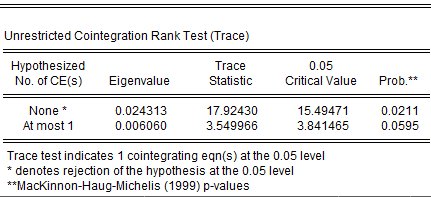
\includegraphics[width=0.6\textwidth]{johansen}
\end{center}
The test for $H_{00}$: ``No cointegration''rejects. The test for $H_{01}$: ``1 cointegration relationship'' accepts. Conclusion: there is one cointegrating relationship. It the latter test had rejected as well, then that would mean that the model is stationary; i.e., the variables aren't integrated in the first place.\newpage
\noindent\textbf{Step 2}: Make a vector autoregression. In the group window, click on \texttt{Proc$\rightarrow$Make Vector Autoregression}.
\begin{center}
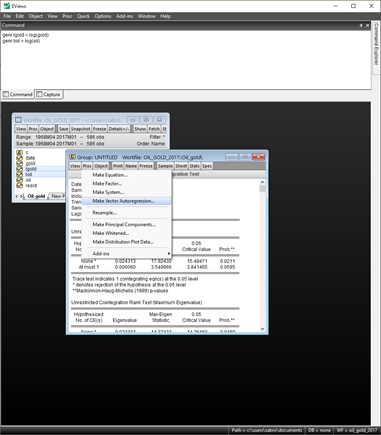
\includegraphics[width=0.7\textwidth]{johanseneviews7}
\end{center}
Choose “Vector Error Correction”, and set the lag interval to match what the criteria found.
\begin{center}
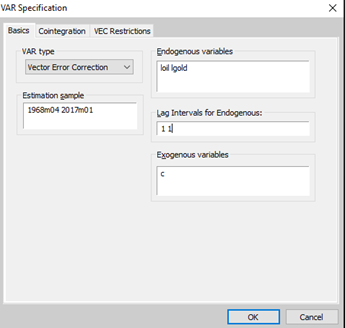
\includegraphics[width=0.4\textwidth]{johanseneviews8}
\end{center}
Go to the \texttt{Cointegration} tab, choose the same model as for the Johansen test (so 3 in this case), and set the number of cointegrating relationships to what the test found (so 1 in this case).
\begin{center}
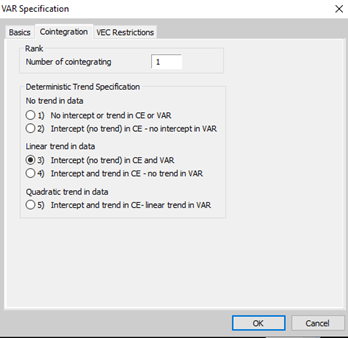
\includegraphics[width=0.4\textwidth]{johanseneviews9}
\end{center}
Result:
\begin{center}
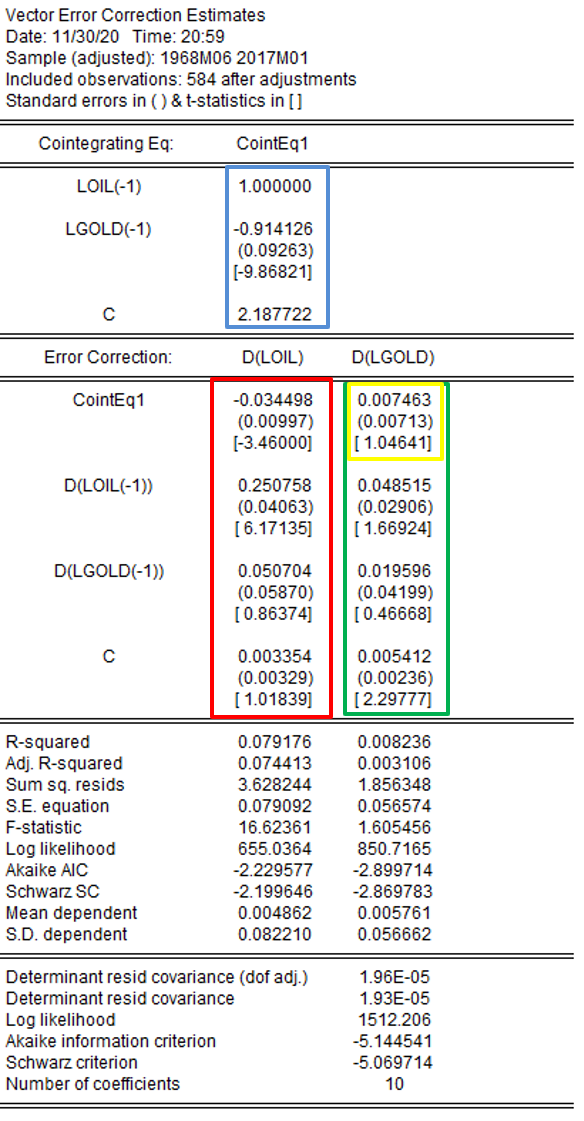
\includegraphics[width=0.4\textwidth]{vecm3_colors}
\end{center}
The red part is the VECM equation for \texttt{LOIL}, the green part is that for \texttt{LGOLD}, and the blue part is the cointegrating relationship. The cointegrating vector is $(1, -0.914)$. The results are remarkably similar to what we found with the Engle-Grander procedure. We could again ignore the equation for \texttt{LGOLD}, because the adjustment coefficient ($\alpha_2$, in yellow) is insignificant ($t$-statistic 1.04). The final model is
{\tiny
\begin{align*}
\Delta \textrm{loil}_t&=0.0034-0.034(\textrm{loil}_{t-1}-0.914\textrm{lgold}_{t-1}+2.19)+0.25\Delta\textrm{loil}_{t-1}+0.05\Delta\textrm{lgold}_{t-1}+e_{1t}\\
\Delta \textrm{lgold}_t&=0.0054-0.007(\textrm{loil}_{t-1}-0.914\textrm{lgold}_{t-1}+2.19)+0.049\Delta\textrm{loil}_{t-1}+0.019\Delta\textrm{lgold}_{t-1}+e_{2t}
\end{align*}}

\end{enumerate}
\item \begin{enumerate}
\item $X_t$ is a random walk, hence $I(1)$. So no, it is not stationary.
\item $Y_t$ depends on $X_t$ if $\beta_2\neq 0$, so it cannot be stationary.
\item Yes, because there exists a linear combination of them that is stationary:
\[
Y_t-\beta_2X_t=\beta_1 +U_{1,t}.
\]
The cointegrating vector is $(1, -\beta_2)$.


\item The goal is to find two equations, one with $\Delta Y_t$ on the LHS, and one with $\Delta X_t.$ Both should have the equilibrium error $Y_{t-1}-\beta_1-\beta_2 X_{t-1}$ on the RHS.

For $Y_t$, we find
\begin{align*}
Y_t&=\beta_1 +\beta_2 X_t+U_{1,t}&|&-Y_{t-1}\\
\Delta Y_t&=-Y_{t-1}+\beta_1+\beta_2X_t+U_{1,t}&|&\pm \beta_2 X_{t-1}\\
\Delta Y_t&=-(Y_{t-1}-\beta_1-\beta_2 X_{t-1})+\beta_2\Delta X_t+U_{1,t}&\\
\Delta Y_t&=\alpha_1(Y_{t-1}-\beta_1-\beta_2X_{t-1})+\beta_2\Delta X_t+U_{1,t},&\\
\intertext{where $\alpha_1=-1$. For $X_t$, }
X_t&=X_{t-1}+U_{2,t}&|&-X_{t-1}\\
\Delta X_t&=U_{2,t}&&\\
\Delta X_t&=0(Y_{t-1}-aX_{t-1})+U_{2,t}\\
\Delta X_t&=\alpha_2(Y_{t-1}-aX_{t-1})+U_{2,t}
\end{align*}
where $\alpha_2=0$. This means that we can treat this as a single-equation ECM.
\end{enumerate}
\end{enumerate}
\end{document} 